%%%%%%%%%%%%%%%%%%%% author.tex %%%%%%%%%%%%%%%%%%%%%%%%%%%%%%%%%%%
%
% sample root file for your "contribution" to a contributed volume
%
% Use this file as a template for your own input.
%
%%%%%%%%%%%%%%%% Springer %%%%%%%%%%%%%%%%%%%%%%%%%%%%%%%%%%


% RECOMMENDED %%%%%%%%%%%%%%%%%%%%%%%%%%%%%%%%%%%%%%%%%%%%%%%%%%%
\documentclass[graybox]{svmult}

% choose options for [] as required from the list
% in the Reference Guide

\usepackage{mathptmx}       % selects Times Roman as basic font
\usepackage{helvet}         % selects Helvetica as sans-serif font
\usepackage{courier}        % selects Courier as typewriter font
\usepackage{type1cm}        % activate if the above 3 fonts are
                            % not available on your system
\usepackage{makeidx}         % allows index generation
\usepackage{graphicx}        % standard LaTeX graphics tool
                             % when including figure files
\usepackage{multicol}        % used for the two-column index
\usepackage[bottom]{footmisc}% places footnotes at page bottom
\usepackage{amsmath,amssymb,latexsym}

%% change footnote numbers to symbols
\renewcommand{\thefootnote}{\fnsymbol{footnote}}
%\newcommand{\bxi}{\ensuremath{\boldsymbol{\xi}}}
%\newcommand{\btheta}{\ensuremath{\boldsymbol{\theta}}}
% see the list of further useful packages
% in the Reference Guide

\makeindex             % used for the subject index
                       % please use the style svind.ist with
                       % your makeindex program

%%%%%%%%%%%%%%%%%%%%%%%%%%%%%%%%%%%%%%%%%%%%%%%%%%%%%%%%%%%%%%%%%%%%%%%%%%%%%%%%%%%%%%%%%

\begin{document}

\section{Numerical Tests}
\label{sec:3}
We implement the Metropolis algorithm in R. Inside the Metropolis
algorithm, we evaluate the  likelihood function using the DTQ method,
which is implemented in C++ as an R package.  Note that all code and
data used in this work is available online
(\url{https://github.com/hbhat4000/sdeinference})---see the ``Rdtq2d'' and
``pursuit2d'' directories.
To test the method, we first consider the SDE
\begin{equation}
\label{eqn:sdeapplication}
\mathrm{d}X_{1,t} =  -\frac{X_{2,t}}{L}\mathrm{d}t + \frac{s_1^2}{L} \mathrm{d}W_{1,t}, \qquad
\mathrm{d}X_{2,t} = \frac{X_{1,t}}{C}\mathrm{d}t + \frac{s_2^2}{C} \mathrm{d}W_{2,t}.
\end{equation}
This system describes a noisy electrical oscillator with one inductor (with inductance $L$) and one capacitor (with capacitance $C$).  The dependent variables $X_{1,t}$ and $X_{2,t}$ represent, respectively, the current and voltage of the circuit at time $t$.

Our goal here is to test the performance of the algorithm using
simulated data.  To generate this data, we start with known values of
the parameters: $L = C = (2 \pi)^{-1}$ and $s_1 =  s_2 = .4/\sqrt{2 \pi}$.
Using a fixed initial condition $(X_{1,0},X_{2,0})$, we then use the
Euler-Maruyama method to step (\ref{eqn:sdeapplication}) forward in
time until a final time $T > 0$.  When we carry out this
time-stepping, we use a step size of $0.001$ and then retain only
those samples at times $t_m = m \Delta t$, from $m = 0$ to $m = M$,
where $M \Delta t = T$.  The simulated data is taken over two periods of the oscillator ($T = 2$) with a full resolution of $\Delta t = 0.01$.  By, for example, taking every other row of this data set, we can obtain data with a resolution of $\Delta t = 0.02$.

Using the samples $\{ \mathbf{x}_m \}_{m=0}^M$ thus constructed, we
run the Metropolis algorithm.  Because capacitance and inductance are
physically constrained to be positive, we set $1/L = \theta_1^2$.  For
the tests presented here, we infer only $\theta_1$, keeping other
parameters fixed at their known values.   For $\theta_1$, we use a diffuse Gaussian prior with mean $0$ and standard deviation $100$.  For the proposal distribution $Z_{N+1}$ in the auxiliary Markov chain, we choose i.i.d. Gaussians with mean $0$ and standard deviation $0.35$.

 When we run the Metropolis algorithm, we discard the first $100$
 samples and retain the next $1000$ samples.  For each value of
 $\Delta t$ and the DTQ time step $h$, we compute both the mean of the
 samples of $\theta_1^2$ and the mode of the kernel density estimate
 of $\theta_1^2$.  We compare these values against the true value of
 the parameter $1/L = 2 \pi$ and record the relative errors as,
 respectively, $e_1$ and $e_2$:
\begin{center}
\begin{tabular}{llll}
$\Delta t$ & $h$ & $e_1$ (relative error of mean) & $e_2$ (relative error of mode) \\ \hline
$0.04$ & $0.04$ & $6.1\%$ & $7.6\%$ \\
$0.04$ & $0.02$ & $0.54\%$ & $6.8\%$ \\
$0.04$ & $0.01$ & $5.1\%$ & $1.1\%$ \\
$0.02$ & $0.02$ & $12\%$ & $14\%$ \\
$0.02$ & $0.01$ & $4.9\%$ & $2.3\%$
\end{tabular}
\end{center}
When $h = \Delta t$, only one step of the method described in Section
\ref{subsec:2-1} is required to go from time $t_m$ to $t_{m+1}$.  This
step does not use any quadrature at all---one merely evaluates
(\ref{eqn:chapman}) using a point mass for the density at time $t_m$.
The resulting likelihood function is a product of Gaussians.  On the
other hand, when $h$ is strictly less than $\Delta t$, we must use
quadrature (i.e., the actual DTQ method) to step forward in time from
$t_m$ to $t_{m+1}$.  Clearly, using the DTQ method to compute the likelihood yields more accurate posteriors than using a purely Gaussian likelihood.

To visualize the results, we present Figure \ref{fig:lcosc}.  The true
value of $1/L = 2 \pi$ is indicated by the dashed black line.  The
posterior mode for $h = 0.01$ is indicated by the solid black line.
The curves are kernel density estimates computed using the posterior
samples described above.
\begin{figure}
\begin{center}
\vspace{-0.55in}
\includegraphics[width=3in,angle=270]{densities.eps}
\end{center}
\vspace{-0.35in}
\caption{We plot kernel density estimates of posterior densities
  $p(\theta_1^2 | \mathbf{x})$.  We use simulated data with  $\Delta t
  = 0.04$, generated as described above.  Each posterior density
  corresponds to a finer DTQ step $h$.  As we take a finer DTQ step
  (i.e., as $h$ decreases), the posterior mode approaches the true
  value indicated by the solid vertical line at $1/L = 2 \pi$.}
\label{fig:lcosc}
\end{figure}

\end{document}